\section{多变量函数的微分学}

\subsection{多变量函数及其连续性}
\subsubsection[平面上的点集]{Point-set}

Point-set $\mathbb{R}$, $\mathbb{R}^n\,n\geq 2$

Recall: Distance on $\mathbb{R}^n$ (Euclidean distance)

\begin{align*}
    d:\,\mathbb{R}^n\times\mathbb{R}^n & \to\mathbb{R}           \\
    (x,y)                              & \mapsto\left|x-y\right|
\end{align*}

\begin{itemize}
    \item Nonnegativity: $d(x,y)\geq 0,\,\forall x,y\in\mathbb{R}^n$; ``$=$'' is archieved iff $x=y$
    \item Symmetic: $d(x,y)=d(y,x)$
    \item Triangle inequality: $d(x,y)\leq d(x,z)+d(z,y),\,\forall x,y,z\in\mathbb{R}^n$
\end{itemize}

\emph{\begin{align*}
        \left|u+v\right|\leq\left|u\right|+\left|v\right| & \iff\left<u+v,u+v\right>\leq \left<u,u\right>+2\left|u\right|\left|v\right|+\left<v,v\right> \\
                                                          & \iff\left<u,v\right>\leq\left|u\right|\left|v\right|\,\text{(Cauchy-Schwarz inequality)}
    \end{align*}}

\begin{define}
    The disc $B\left(M_0,r\right)=\left\{M\in\mathbb{R}^n\mid d\left(M,M_0\right)<r\right\}$ is called a disc-neighborhood of $M_0$, which is also denoted by $B_r\left(M_0\right)$. $B^-\left(M_0,r\right)=B\left(M_0,r\right)\setminus\left\{M_0\right\}$ is called punctured disc.
\end{define}

\begin{define}
    $E\subseteq\mathbb{R}^n$ is called bounded if $E\subseteq B(0,R)$ for some $R>0$, and the number
    $$
        \operatorname{diam}E\triangleq\sup\left\{d\left(M',M''\right)\mid M',M''\in E\right\}
    $$
    is called the diameter of $E$.
\end{define}

\begin{define}
    Let $E\subseteq\mathbb{R}^n$ and $E^C=\mathbb{R}^n\setminus E$ be its complement.
    \begin{enumerate}
        \item If $\exists r>0$, s.t. $B(M,r)\subseteq E$, then $M$ is called an \emph{interior point 内点} of $E$.
        \item If $\exists r>0$, s.t. $B(M,r)\subseteq E^C$, then $M$ is called an \emph{exterior point 外点} of $E$.
        \item If $\exists r>0,\,B(M,r)\cap E\neq\emptyset,\,B(M,r)\cap E^C\neq\emptyset$, then $M$ is called a \emph{boundary point 边界点} of $E$.
              \begin{center}
                  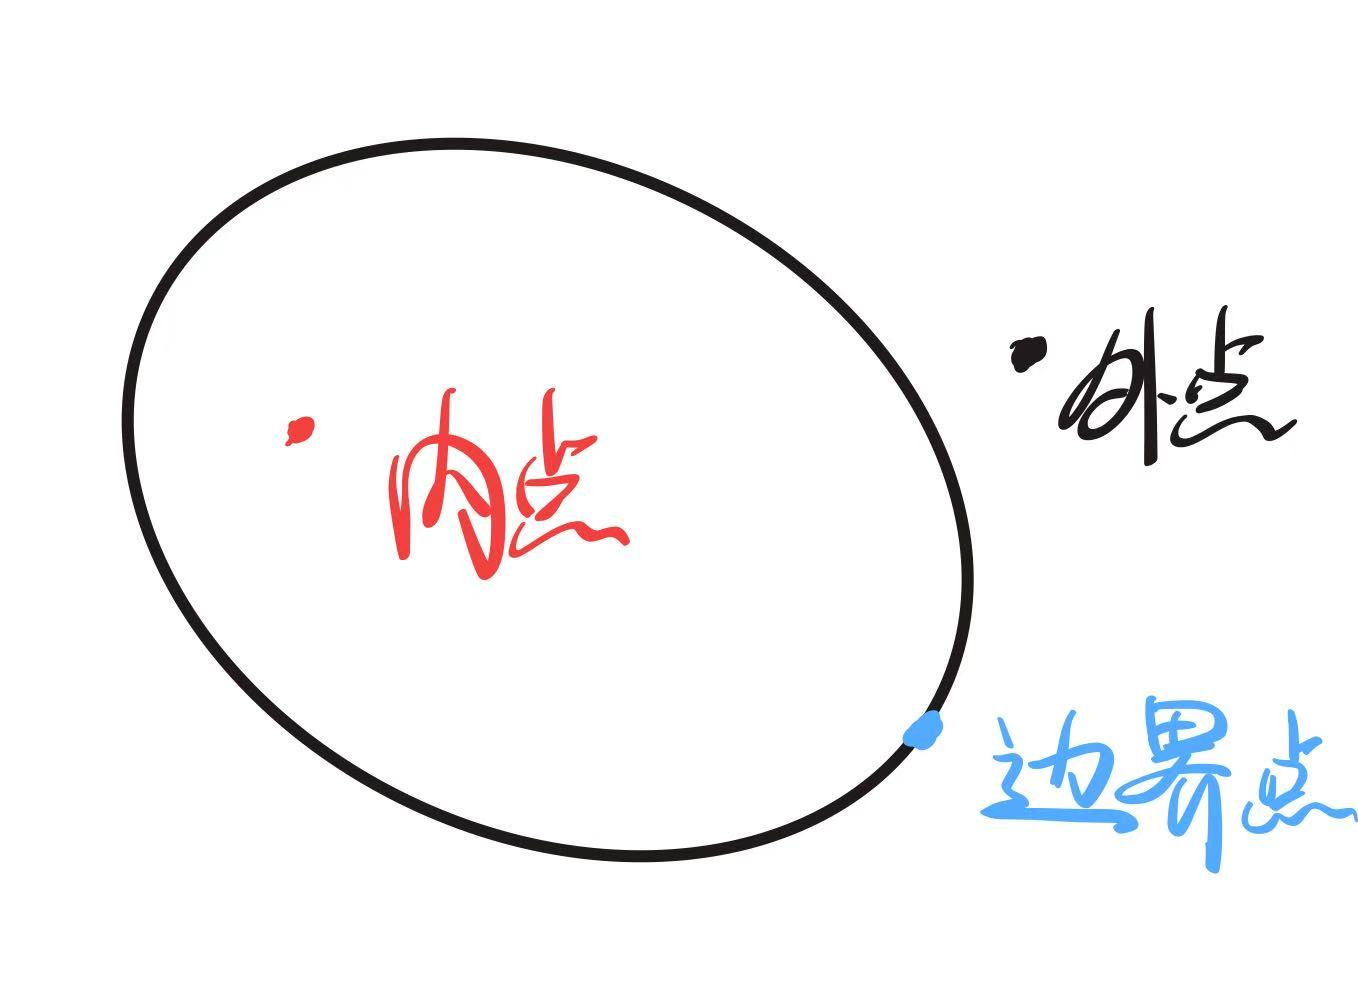
\includegraphics[height=3cm]{chapters/09/01/0101}
              \end{center}
        \item $\mathring{E}=\left\{M\in\mathbb{R}^n\mid M\text{ is an interior point of }E\right\}$, is called the \emph{interior 内部} of $E$.
        \item \allbold{$\partial$: partial}\quad$\partial E=\left\{M\in\mathbb{R}^n\mid M\text{ is a boundary point of }E\right\}$, is called the boundary of $E$.
        \item If $\exists r>0$, s.t. $B(M,r)\cap E=\{M\}$, then $M$ is called an \emph{isolated point 孤立点}.
        \item If $\forall r>0,\,B^-(M,r)\cap E\neq\emptyset$, then $M$ is called a \emph{accumulation point 聚点}.

              $\overline{E}=E\cup\partial E$, is called the \emph{closure 闭包} of $E$.
    \end{enumerate}
\end{define}

\begin{rmk}
    \begin{enumerate}
        \item Interior point $implies$ accumulation point
              \begin{enumerate}
                  \item $M\in E\implies M$ is an accumulation point
                  \item $M\not\in E\implies$ any punctured disc neigh. contains points in $E\implies$ accumulation
              \end{enumerate}
        \item boundary point $\implies$ either isolated point or accumulation point

              \emph{boundary point $+$ non-isolated $\implies$ accumulation point}
    \end{enumerate}
\end{rmk}

\begin{define}
    Let $\left\{M_n\right\}$ be a sequence of points on $\mathbb{R}^2$, and $M_0\in\mathbb{R}^2$. If $\lim_{n\to+\infty}d\left(M_n,M_0\right)=0$, we say $M_n$ converges to $M_0$ (as $n\to+\infty$), also denoted by $\lim_{n\to+\infty}M_n=M_0$
\end{define}

$M_n=\binom{x_n}{y_n},\,M_0=\binom{x_0}{y_0}$, then $\lim_{n\to+\infty}M_n=M_0\iff\lim_{n\to+\infty}x_n=x_0$, and $\lim_{n\to+\infty}y_n=y_0$

\emph{i.e. $\sqrt{\left(x_n-x_0\right)^2+\left(y_n-y_0\right)^2}\to 0,\,\left|x_n-x_0\right|,\left|y_n-y_0\right|\leq d\left(M_n,M_0\right)\leq\left|x_n-x_0\right|+\left|y_n-y_0\right|$}

\begin{mdframed}
    A sequence of points $\left\{M_n\right\}$ is called a Cauchy Seq. if
    $$\forall\varepsilon>0,\,\exists N=N(\varepsilon)\in\mathbb{N}_+\text{, s.t. }\forall n,m>N,\,d\left(M_n,M_m\right)<\varepsilon$$
    \begin{thm}
        \begin{enumerate}
            \item \emph{(Completeness)} All Cauchy seq. in $\mathbb{R}^n$ has convergent subseq.
            \item \emph{(Bolzano-Weierstrass Thm.)} All bounded seq. in $\mathbb{R}^n$ has convergent subseq.
        \end{enumerate}
    \end{thm}
\end{mdframed}

\begin{define}[Open set / Closed set]
    If $E=\mathring{E}$, we say $E$ is open. If $E^C$ is open, we say $E$ is closed.
\end{define}

\begin{example}
    Disc-neighborhood $B(M,r)=\left\{O\in\mathbb{R}^n\mid d(P,M)<r\right\}$ is open.
\end{example}

$\forall P\in B(M,r),\,d(P,M)<r$\\
$\implies B\left(P,r-d(P,M)\right)\subseteq B(M,r)$\\
$\left(d(Q,M)\leq d(Q,P)+d(P,M)<\left(r-d(P,M)\right)+d(P,M)\right)=r,\,\forall Q\in B\left(P,r-d(P,M)\right)$\\
$\implies B(P,r)$ is open, $B(P,r)^C$ closed.\\
$\partial B(M,r)=\left\{P\in\mathbb{R}^n\mid\boxed{d(P,M)=r}\right\}=S(M,r)\leftarrow\text{\emph{Sphere}}$

\begin{prop}
    \begin{enumerate}
        \item $E_1,E_2$ open $\implies E_1\cap E_2$ is open.\\
              (If $E_1,\dots,E_n$ open, then $E_1\cap\cdots\cap E_n$ is open)

              If $\left\{E_\alpha\right\}_{\alpha\in\Lambda}$ is a \emph{family 族} of open sets, then $\bigcup_{\alpha\in\Lambda}E_\alpha$ is open.

              \emph{\begin{flalign*}
                      \impliedby \forall x\in\bigcup_{\alpha\in\Lambda}E_\alpha & \implies x\in E_\alpha\text{ for some }\alpha\in\Lambda    & \\
                                                                                & \implies\exists r>0\text{ s.t. }B(x,r)\subseteq E_\alpha   & \\
                                                                                & \implies B(x,r)\subseteq\bigcup_{\alpha\in\Lambda}E_\alpha &
                  \end{flalign*}}

              \boxed{\bigcap_{n=1}^{\infty}B\left(0,\frac{1}{n}\right)=\{0\}\text{ not open}}
        \item $E_1,E_2$ closed $\implies E_1\cup E_2$ is closed.\\
              (If $E_1,\dots,E_n$ closed, then $E_1\cup\cdots\cup E_n$ is closed)

              If $\left\{E_\alpha\right\}_{\alpha\in\Lambda}$ is a family of closed sets, then $\bigcap_{\alpha\in\Lambda}E_\alpha$ is closed.
        \item $E$ is open iff $E\cap\partial E=\emptyset$, i.e. $\partial E\subseteq E^C$
        \item $\underset{\substack{\Downarrow\\E^C\text{ open }\implies E^C\cap\partial\left(E^C\right)=E^C\cap\partial E=\emptyset}}{E\text{ is closed iff }E^C\cap\partial E=\emptyset}$, i.e. $\partial E\subseteq E$
        \item $E$ is closed iff it contains all of its accumulation points.
    \end{enumerate}
\end{prop}

\begin{pf}
    \begin{enumerate}
        \item $\forall x\in E_1\cap E_2,\,\exists r_1,r_2>0$, s.t. $B(x,r_1)\subseteq E_1,\,B(x,r_2)\subseteq E_2$\\
              $\implies B\left(x,\min\left\{r_1,r_2\right\}\right)\subseteq E_1\cap E_2$
        \item \allbold{$\left(E_1\cup E_2\right)^C=E_1^C\cap E_2^C$}\\
              $\left(\bigcap_{\alpha\in\Lambda}E_\alpha\right)^C=\bigcup_{\alpha\in\Lambda}E_\alpha^C$

              \allbold{\begin{align*}
                      x\in\left(\bigcap_{\alpha\in\Lambda}E_\alpha\right)^C & \iff x\not\in\bigcap_{\alpha\in\Lambda}E_\alpha                                                            \\
                                                                            & \iff x\not\in E_\alpha\text{ for some }\alpha\in\Lambda                                                    \\
                                                                            & \iff x\in E_\alpha^C\text{ for some }\alpha\in\Lambda\text{ i.e. }x\in\bigcup_{\alpha\in\Lambda}E_\alpha^C
                  \end{align*}}
        \item \emph{``$\implies$''} $E$ is open $\implies\forall x\in E,\,\exists r>0$ s.t. $B(x,r)\subseteq E\implies x\not\in\partial E\implies\partial E\subset E^C$

              \emph{``$\impliedby$'' If $\partial E\cap E=\emptyset$, then $\forall x\in E\implies x\not\in\partial E\xrightarrow{\text{反证}}\exists r>0$ s.t. $B(x,r)\subseteq E\implies x$ is an interior $\implies E$ open.}

              \setcounter{enumi}{4}

        \item ``$\implies$'' $E$ closed, $\boxed{x\text{ is an accumulation point}}$, we want to prove $x\in E$ by contradiction.

              Suppose $x\not\in E$, then $x\in E^C$ which is open. Then $B(x,r)\subseteq E^C$ for some $r>0$, so $x$ is not accumulation point of $E$, it's a contradiction.

              Therefore, $x\in E$.

              ``$\impliedby$'' $\forall x\in E^C$, then $x$ is not accumulation point by assumption.

              $\implies\exists r>0$ s.t. $B^-(x,r)\cap E=\emptyset\implies B^-(x,r)\subseteq E^C$\\
              $\implies B(x,r)\subseteq E^C\implies E^C$ open $\implies E$ closed.
    \end{enumerate}
\end{pf}

\begin{define}[Connectivity]
    A subset $E\subseteq \mathbb{R}^n$ is called \emph{connected} if for any \emph{nontrivial} ($A,B\neq\emptyset$) decomposition $E=\underset{\text{\textbf{disjoint set}}}{A\sqcup B}$, either $\underset{\text{\allbold{$
                        \begin{aligned}x\in A\cap\overline{B}\neq\emptyset & \implies x\in\overline{B}\setminus B                                    \\
                                                   & \implies x\in(\partial B)\cap B^C                                       \\
                                                   & \implies x\text{ is accumulation of }B,\,B\cap\overline{A}\neq\emptyset
                        \end{aligned}$}}
        }{A\text{ contains some accumulation points of }B}$
\end{define}

\begin{define}[Path-connected 道路连通]
    If $\forall P,Q\in E,\,\exists$ continuous map
    $$\begin{aligned}
            \gamma:\,[0,1] & \to \mathbb{R}^n      \\
            t              & \mapsto\begin{pmatrix}
                                        x_1(t) \\
                                        \vdots \\
                                        x_n(t)
                                    \end{pmatrix}
        \end{aligned}$$
    s.t.$\gamma\left([0,1]\right)\subseteq E$, and $\gamma(0)=P,\,\gamma(1)=Q$
\end{define}

\begin{example}
    $E=\left\{(0,y)\mid -1\leq y\leq 1\right\}\cup\left\{\left(x,\sin\frac{1}{x}\mid x\in(0,1]\right)\right\}$ \textbf{Not path connected, but it is connected}
\end{example}

\begin{thm}
    If $E$ is path-connected, then $E$ is connected.
\end{thm}

\begin{pf}
    Argue by contradiction. Suppose $E$ is not connected / disconnected. Then $A,B\neq\emptyset,\,A\cap B=\emptyset$, s.t. $A\sqcup B=E$ and $A\cap\overline{B}=\emptyset,\,B\cap\overline{A}=\emptyset$. By path-connectedness, take $x\in A,\,y\in B,\,\gamma:\,[0,1]\to\mathbb{R}^n$, path connecting $x$ and $y$ in $E$ to $\triangleq\sup\left\{t\in[0,1]\mid r(t)\in A\right\}\neq\emptyset$

    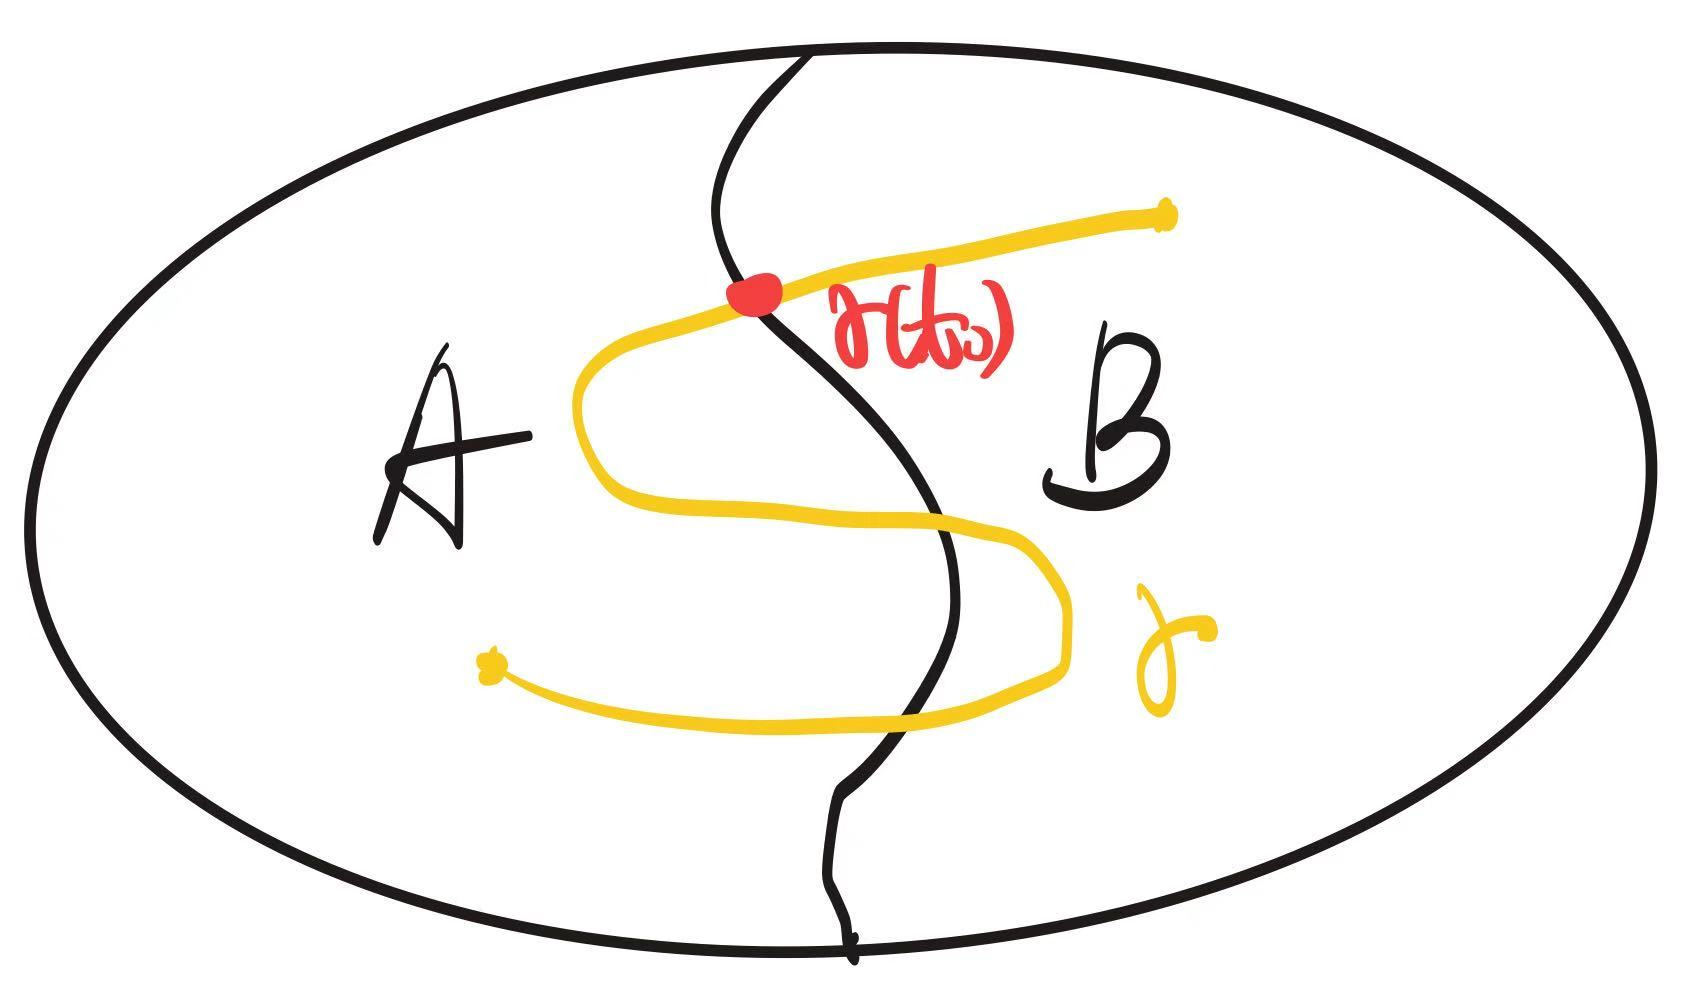
\includegraphics[height=2cm]{chapters/09/01/0102}

    \allbold{\begin{enumerate}
            \item $r\left(t_0\right)\in A\implies t_0\neq 1,\,\forall t>t_0,\,r(t)\in B$\\
                  $\implies r\left(t_0\right)$ is accumulation point of $B$\\
                  $\implies r\left(t_0\right)\in\overline{B}\subseteq A^C$, contradiction.
            \item $r\left(t_0\right)\in B\implies\exists t_n\nearrow t_0$ s.t. $r\left(t_n\right)\in A$\\
                  $\implies r\left(t_0\right)$ is accumulation point of $A$\\
                  $\implies r\left(t_0\right)\in\overline{A}\subseteq B^C$, contradiction.
        \end{enumerate}}
\end{pf}

\begin{rmk}
    Open set is connected iff it is path-connected.

    \allbold{(Pick any $P\in X$, define
        $$U=\left\{Q\in X\mid Q\text{ and }P\text{ can be connected by a path in }X\right\},$$
        prove $U=X$)}

    \begin{center}
        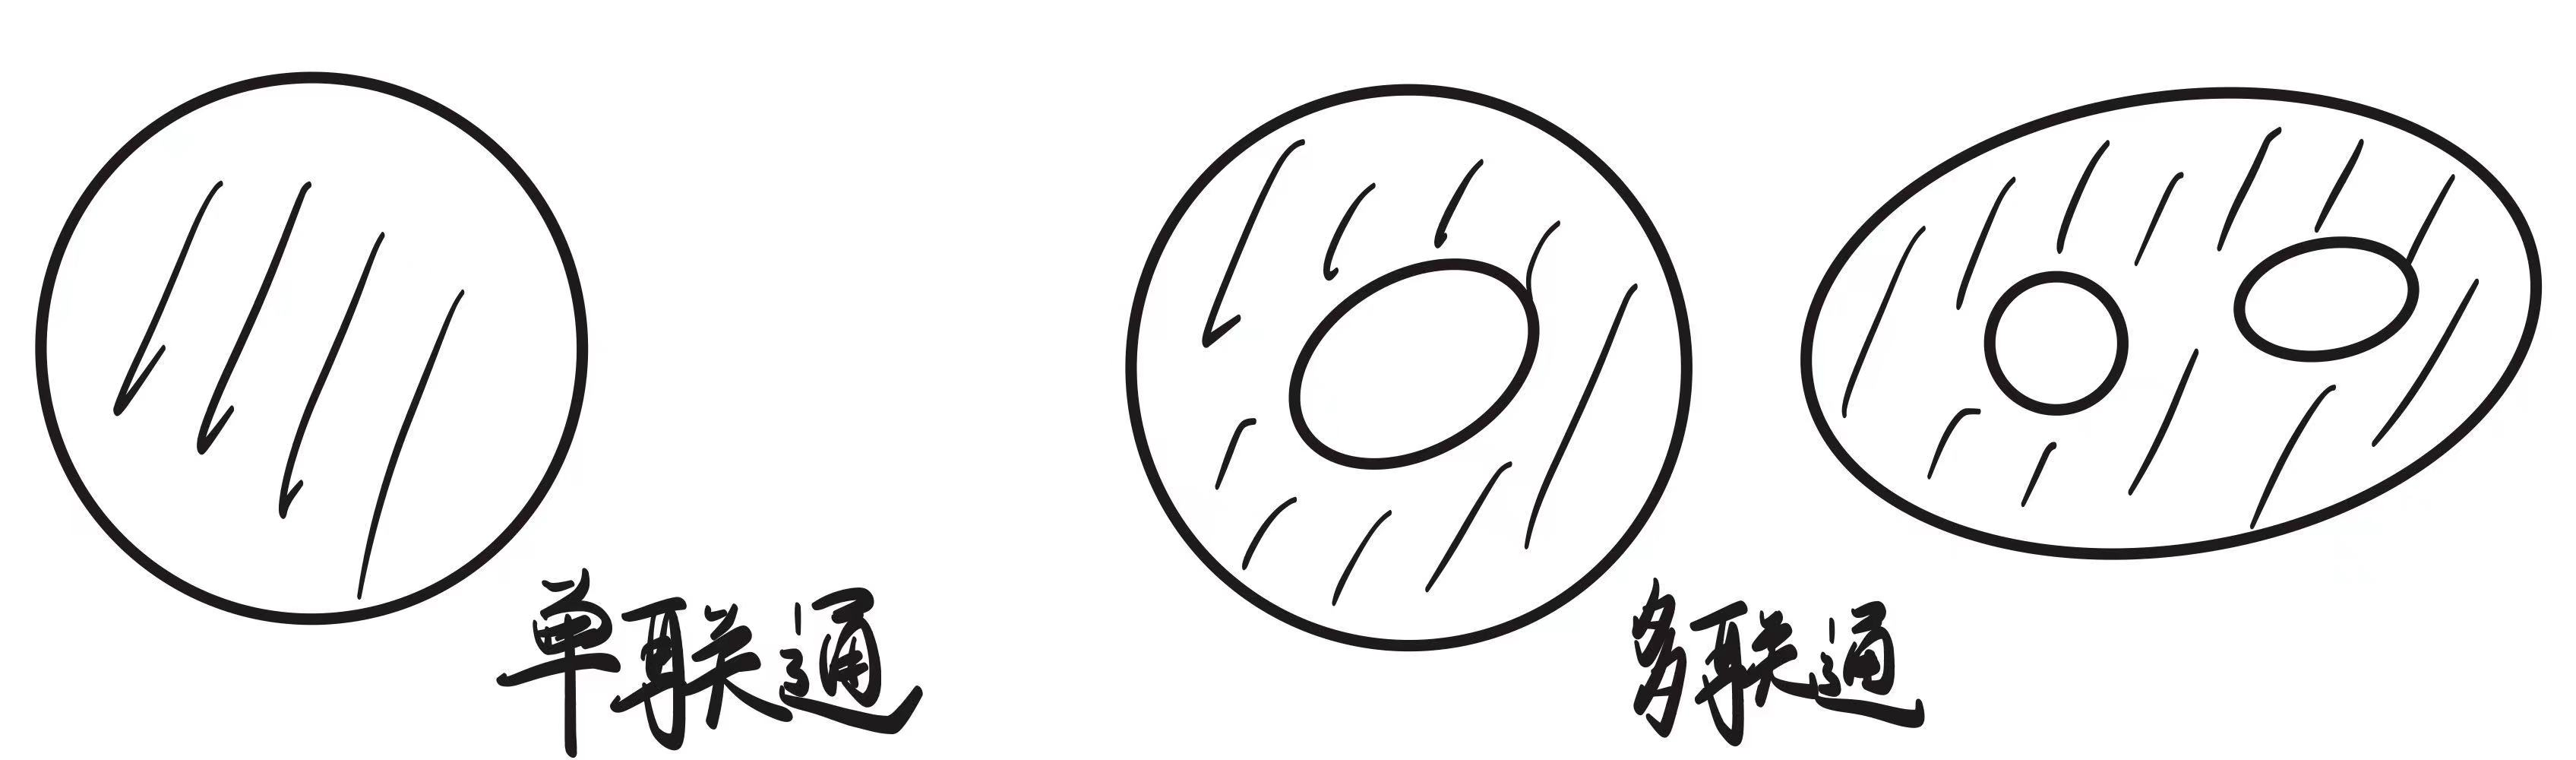
\includegraphics[height=3cm]{chapters/09/01/0103}
    \end{center}
\end{rmk}

\begin{define}[Single Curve]
    If a curve: $\gamma:\,[\alpha,\beta]\to\mathbb{R}^2$ satisifies $\gamma\left(t_1\right)\neq\gamma\left(t_2\right)$ for any $\alpha\leq t_1<t_2\leq\beta$, then $\gamma$ is called a single curve. \emph{(Not self- intersection)}\raisebox{-1\height}{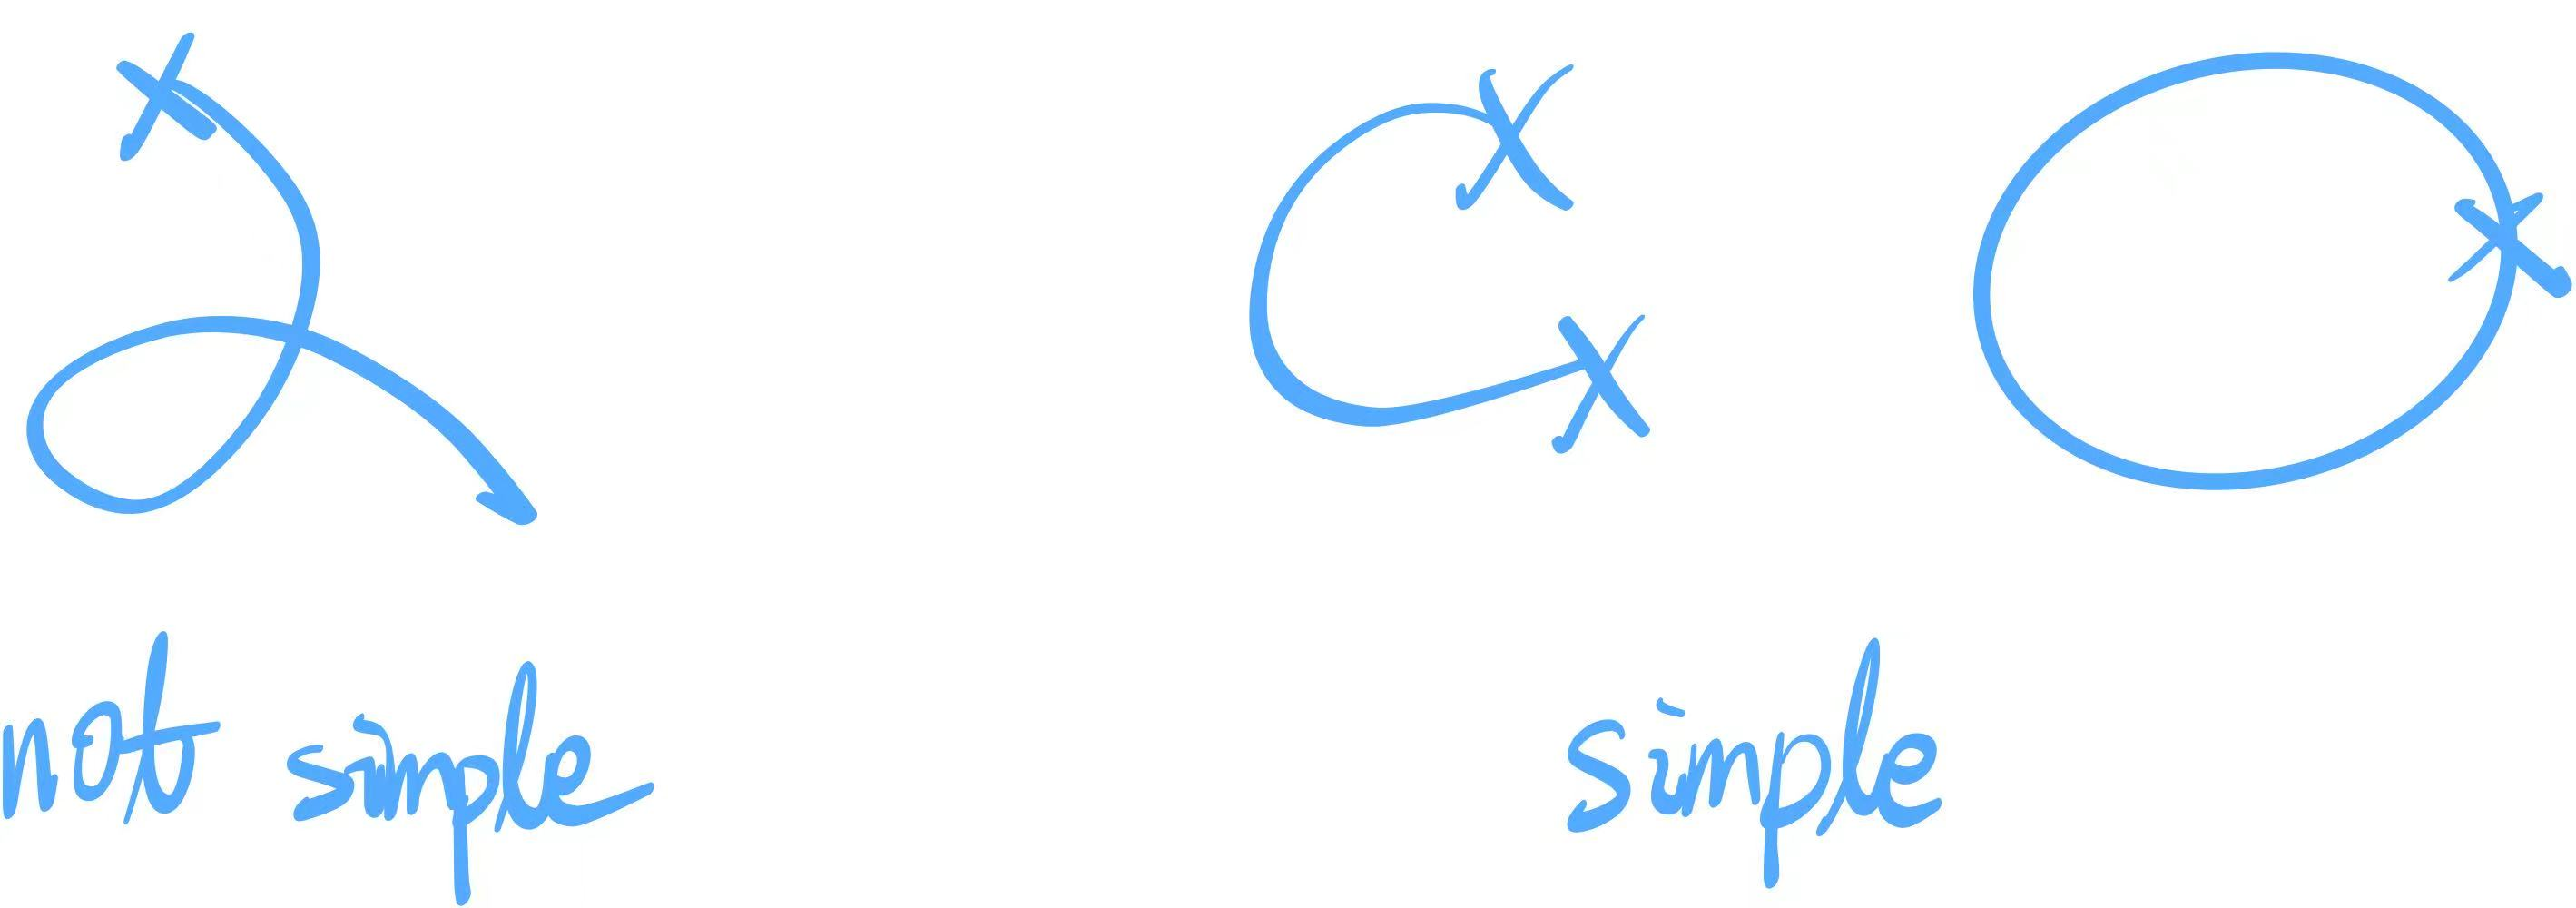
\includegraphics[height=2cm]{chapters/09/01/0104}}
\end{define}

\begin{define}[Loop / Closed Curve]
    If the curve $\gamma:\,[\alpha,\beta]\to\mathbb{R}^2$ has the same starting and ending point, i.e. $\gamma(\alpha)=\gamma(\beta)$, then $\gamma$ is called a loop, or a closed curve.\raisebox{-1\height}{
\includegraphics[height=1cm]{chapters/09/01/0105}}
\end{define}

\begin{thm}[Jordan Curve Theorem]
    Any simple closed curve $\gamma$ on $\mathbb{R}^2$ divides $\mathbb{R}^2$ into two open connected sets, one is bounded called the interior part of $\gamma$, and the other which is unbounded called the exterior part of $\gamma$.\raisebox{-1\height}{
\includegraphics[height=2cm]{chapters/09/01/0106}}
\end{thm}

环面：\raisebox{-0.5\height}{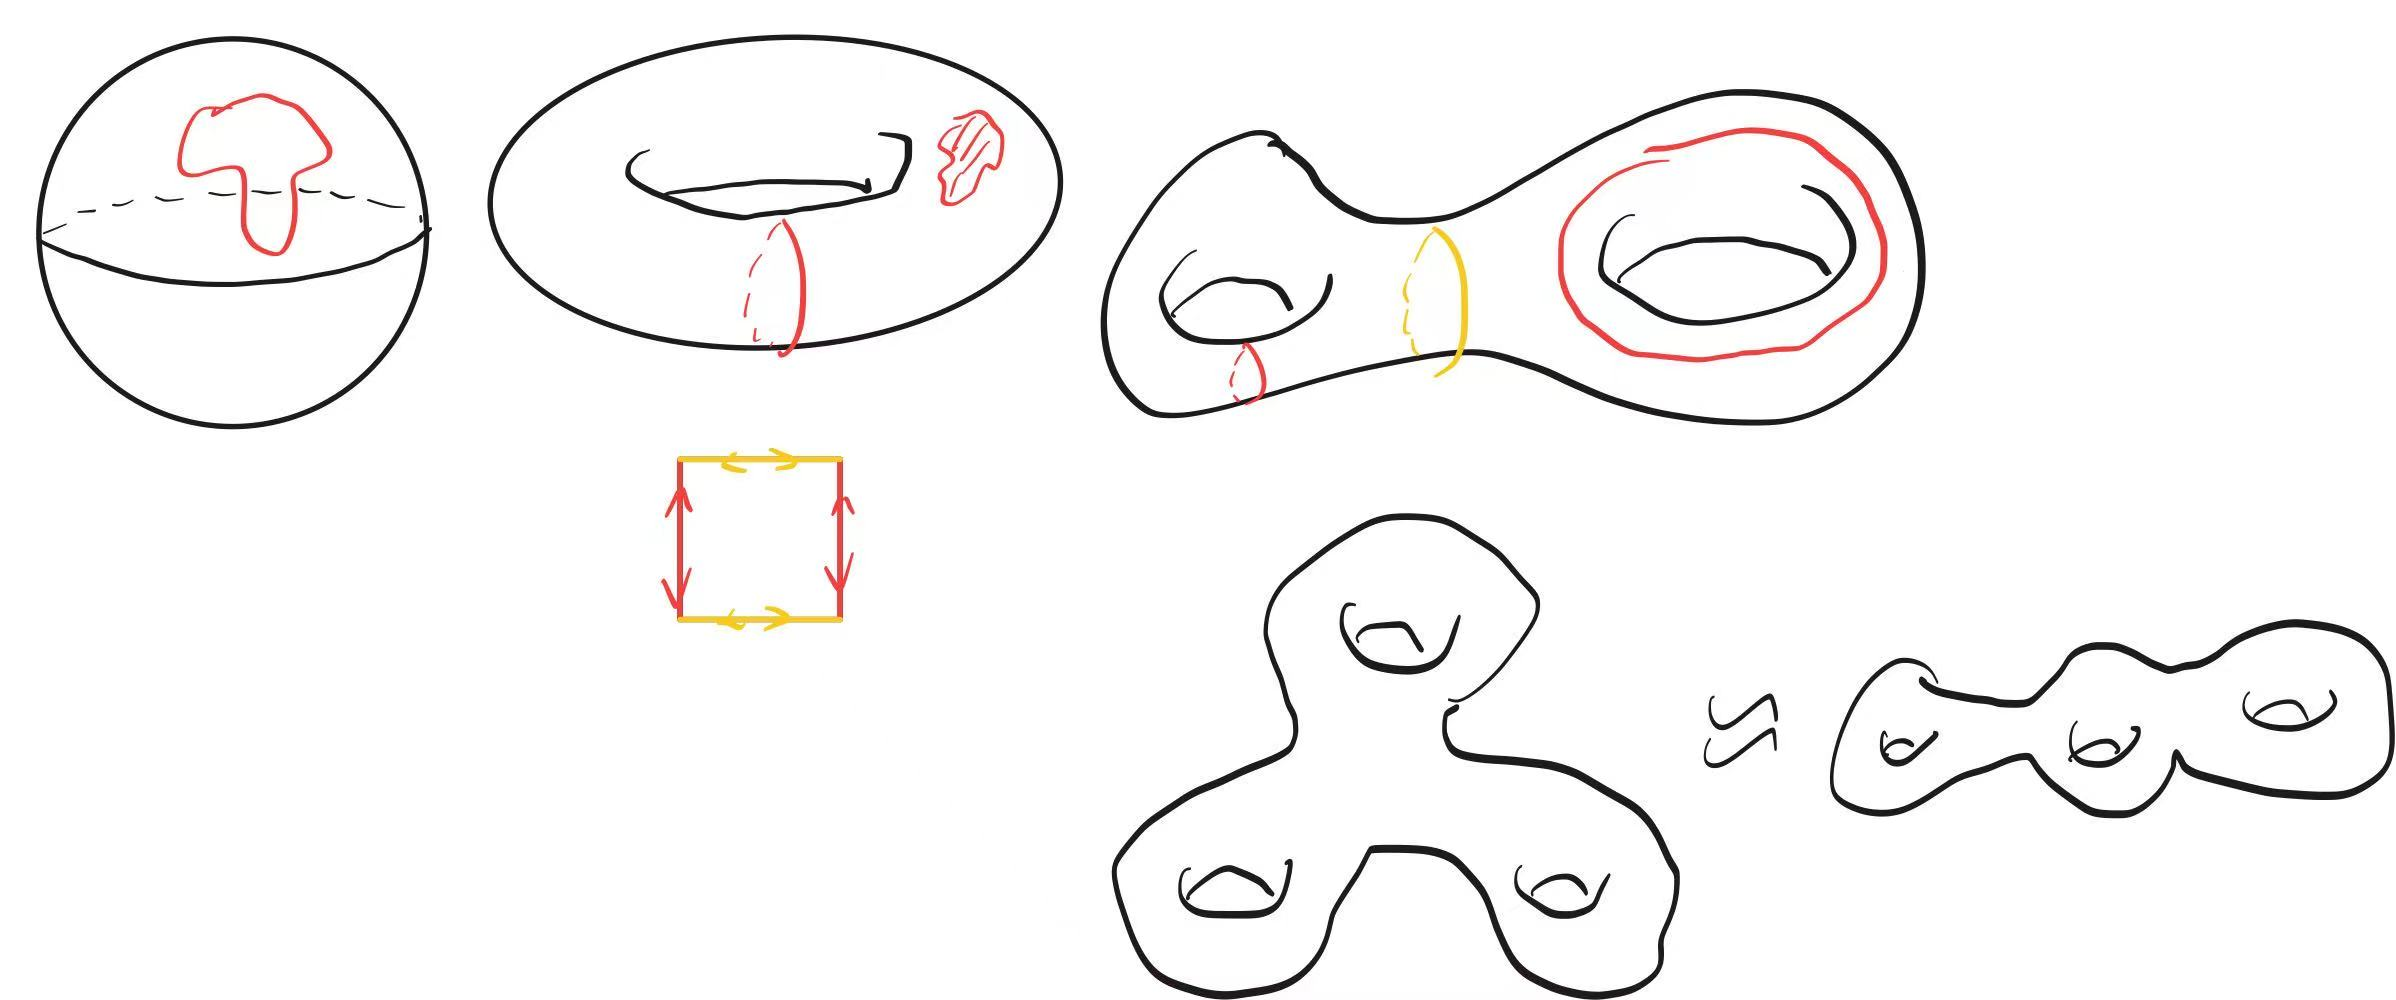
\includegraphics[height=5cm]{chapters/09/01/0107}}

If the \emph{interior point} of any single closed curve in $D$ (connected open set) is contained in $D$, then $D$ is called \textbf{simply-connected}. Otherwise, it is called multi-connected.

\begin{rmk}
    Topological definition (depends on the crucial notion homotopy 同伦)

    For $\mathbb{R}^2$, any loop is \emph{null-homotopic 零伦}, i.e. it is homotopic to a trivial loop.

    \emph{$\Pi_1(x)$ 基本群}
\end{rmk}